% !TEX TS-program = pdflatex
% !TEX encoding = UTF-8 Unicode

% This is a simple template for a LaTeX document using the "article" class.
% See "book", "report", "letter" for other types of document.

\documentclass[11pt]{article} % use larger type; default would be 10pt

\usepackage[utf8]{inputenc} % set input encoding (not needed with XeLaTeX)

%%% Examples of Article customizations
% These packages are optional, depending whether you want the features they provide.
% See the LaTeX Companion or other references for full information.

%%% PAGE DIMENSIONS
\usepackage{geometry} % to change the page dimensions
\geometry{a4paper} % or letterpaper (US) or a5paper or....
% \geometry{margin=2in} % for example, change the margins to 2 inches all round
% \geometry{landscape} % set up the page for landscape
%   read geometry.pdf for detailed page layout information

\usepackage{graphicx} % support the \includegraphics command and options

% \usepackage[parfill]{parskip} % Activate to begin paragraphs with an empty line rather than an indent

%%% PACKAGES
\usepackage{booktabs} % for much better looking tables
\usepackage{array} % for better arrays (eg matrices) in maths
\usepackage{paralist} % very flexible & customisable lists (eg. enumerate/itemize, etc.)
\usepackage{verbatim} % adds environment for commenting out blocks of text & for better verbatim
\usepackage{subfig} % make it possible to include more than one captioned figure/table in a single float
% These packages are all incorporated in the memoir class to one degree or another...

%%% HEADERS & FOOTERS
\usepackage{fancyhdr} % This should be set AFTER setting up the page geometry
\pagestyle{fancy} % options: empty , plain , fancy
\renewcommand{\headrulewidth}{0pt} % customise the layout...
\lhead{}\chead{}\rhead{}
\lfoot{}\cfoot{\thepage}\rfoot{}

%%% SECTION TITLE APPEARANCE
\usepackage{sectsty}
\allsectionsfont{\sffamily\mdseries\upshape} % (See the fntguide.pdf for font help)
% (This matches ConTeXt defaults)

%%% ToC (table of contents) APPEARANCE
\usepackage[nottoc,notlof,notlot]{tocbibind} % Put the bibliography in the ToC
\usepackage[titles,subfigure]{tocloft} % Alter the style of the Table of Contents
\renewcommand{\cftsecfont}{\rmfamily\mdseries\upshape}
\renewcommand{\cftsecpagefont}{\rmfamily\mdseries\upshape} % No bold!

%%% END Article customizations

%%% The "real" document content comes below...

\title{LiveIntent BI challenge}
\author{Julie Sainmont}
%\date{} % Activate to display a given date or no date (if empty),
         % otherwise the current date is printed 

\begin{document}
\maketitle

\section{Purpose}
LiveIntent is currently purchasing a license from LiveRamp to use their set of identifiers to provide services to other partners. However LiveIntent is considering whether it should replace that partnership with one of more other partners. The suggested new partners are Audience Accuity and TowerData. This report investigate if the suggested change is supported by the data, and will indeed provide LiveIntent with a better coverage of identifiers at its disposal. \\

% section -Assessment
\section{Assessment of the identifier's coverage and the volume and performance of the licenses}
\begin{figure}[h!]
  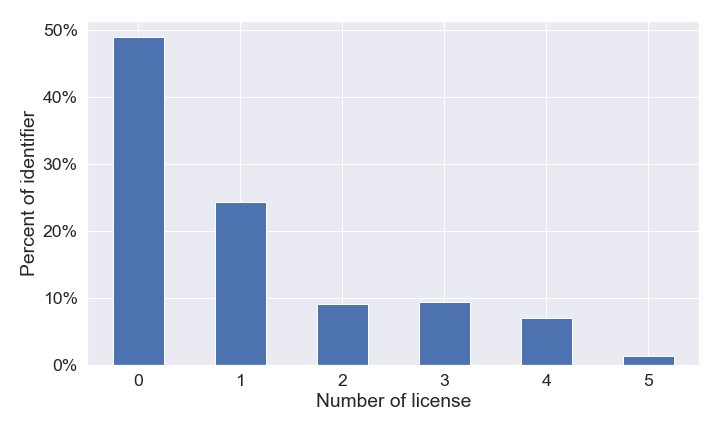
\includegraphics[width=0.8\linewidth]{../outputs/distribution_identifier_license.png}
  \caption{Distribution of the number of licenses covering the identifiers.}
  \label{fig:nr_licences_per_identifier}
\end{figure}

\begin{figure}[h!]
  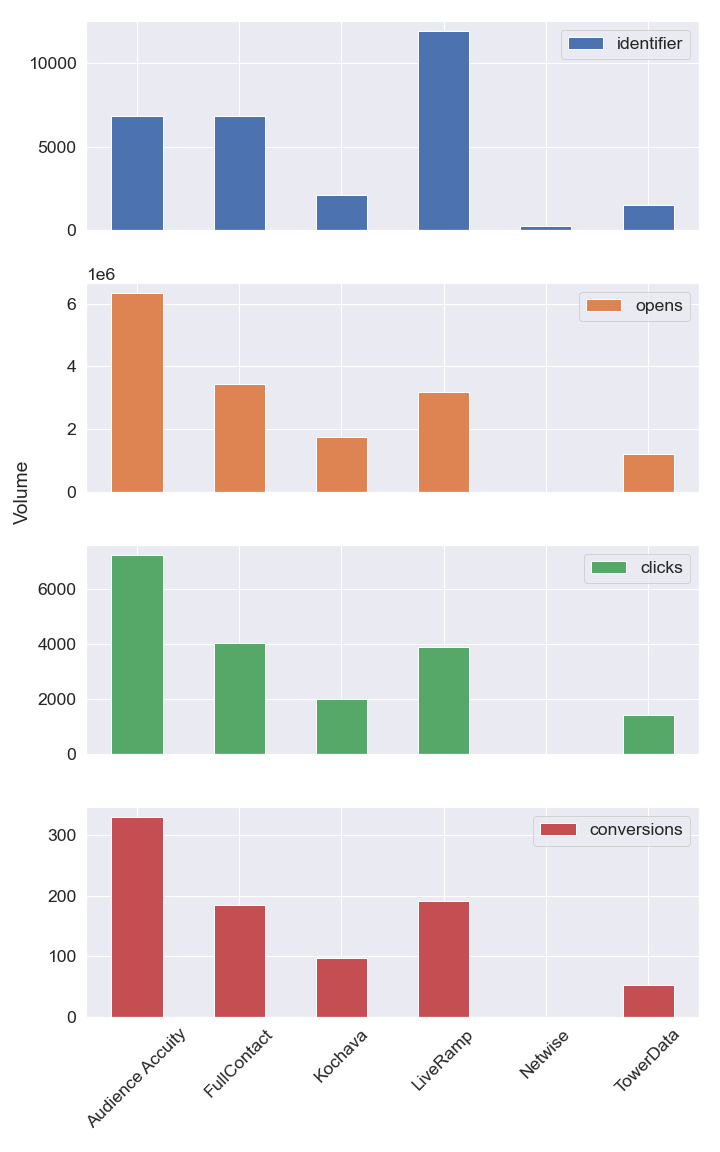
\includegraphics[width=0.8\linewidth]{../outputs/volume_per_license.png}
  \caption{Volume of identifier and activities per license.}
  \label{fig:volume_per_license}
\end{figure}

\begin{figure}[h!]
  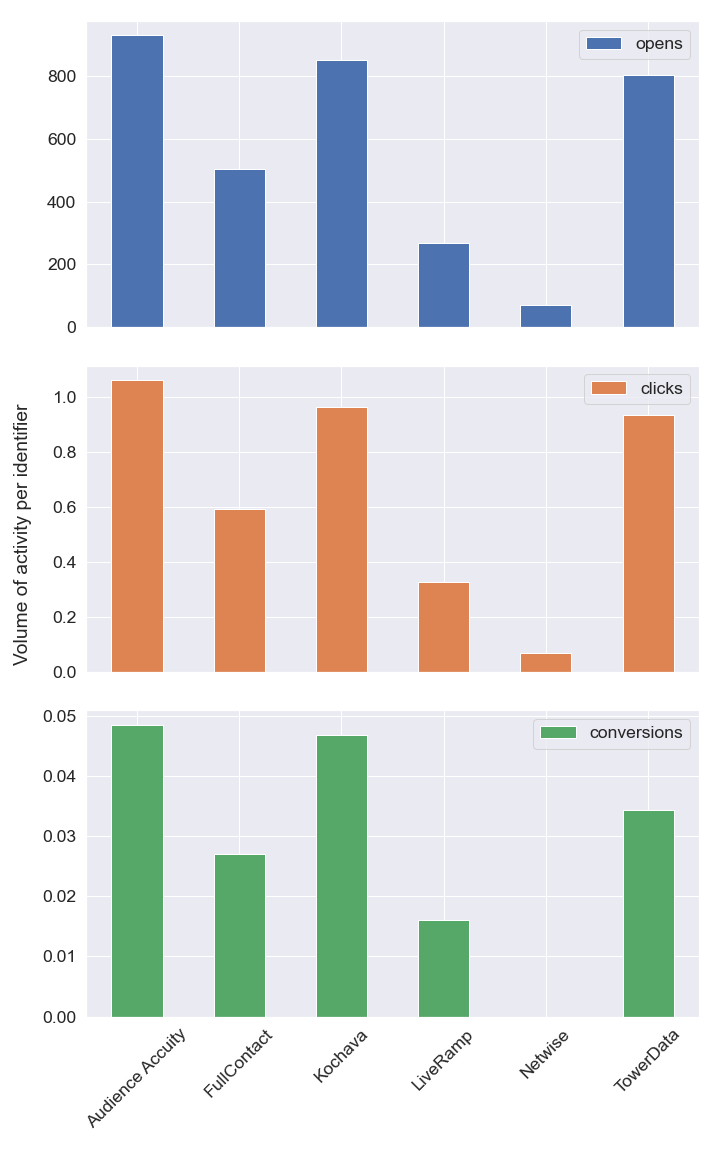
\includegraphics[width=0.8\linewidth]{../outputs/volume_per_identifier_per_license.png}
  \caption{Volume of identifier and activities per license.}
  \label{fig:volume_per_id_per_license}
\end{figure}

From the provided dataset, we can see that about nearly 50\% of the dataset is not covered by any licenses, 24\% is covered only by one license, and a bit more than 26\% is covered by 2 or more licenses (figure \ref{fig:nr_licences_per_identifier}).\\

When focusing on the different licenses, we can see that LiveRamp has the highest coverage of identifiers (close to 12000, figure \ref{fig:volume_per_license}), however the identifiers covered by Audience Accuity show more activities in numbers of opens, clicks and conversions suggesting that even though Audience Accuity is a bit smaller it could perform better. This is confirmed when looking at the ratio between the identifier's activity versus their volume (figure \ref{fig:volume_per_id_per_license}) where LiveRamp has one of the poorest performance. Kochava and Audience Accuity are leading the group followed closely by TowerData.\\

FullContact has a fairly close volume of identifier coverage than Audience Accuity but show only about half the quantity of activities (figure \ref{fig:volume_per_license} and \ref{fig:volume_per_id_per_license}). Netwise is from far the smallest of all licenses investigated.\\


Audience Accuity seems to be a good choice of licenses. it could be interesting to combine it with one of two other licenses to compensate the smaller volume of identifier covered. Given that identifiers can be covered by several licenses it is crucial to ensure the smallest overlap between the purchased license.\\

% section -Overlap of the licenses
\clearpage
\newpage
\section{Overlap of the licenses}
The Kochava licenses has a large percentage of overlap with LiveRamp, Audience Accuity and FullContact (94\%, 97\% and 97\% respectively, figure \ref{fig:venn_matrix} and \ref{fig:heatmap_overlap}). Given that it is also the smallest of the 3 licenses, it is not worth considering further. Netwise, although very small, has very limited overlap with all the other licenses and could therefore be a good complement to the chosen license set (only 19\% of the identifiers are covered by Audience Accuity, and it is below 4\% and 1\% for TowerData and LiveRamp respectively).
\begin{figure}[h!]
  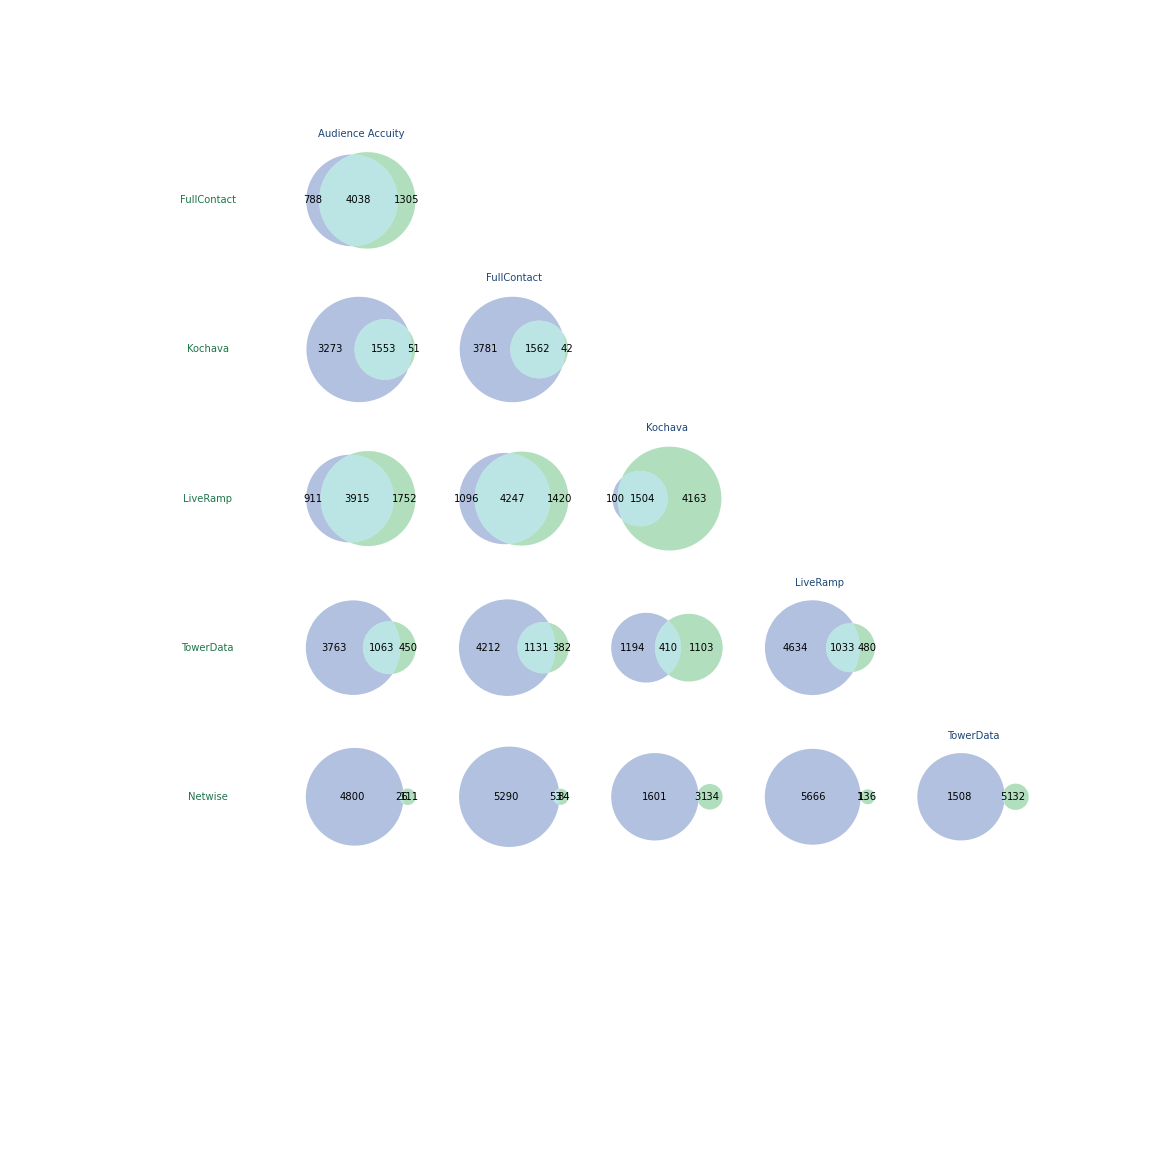
\includegraphics[width=1.1\linewidth]{../outputs/venn_matrix.png}
  \caption{Matrix of the overlap of identifier covered across the licenses.}
  \label{fig:venn_matrix}
\end{figure}

\begin{figure}[h!]
  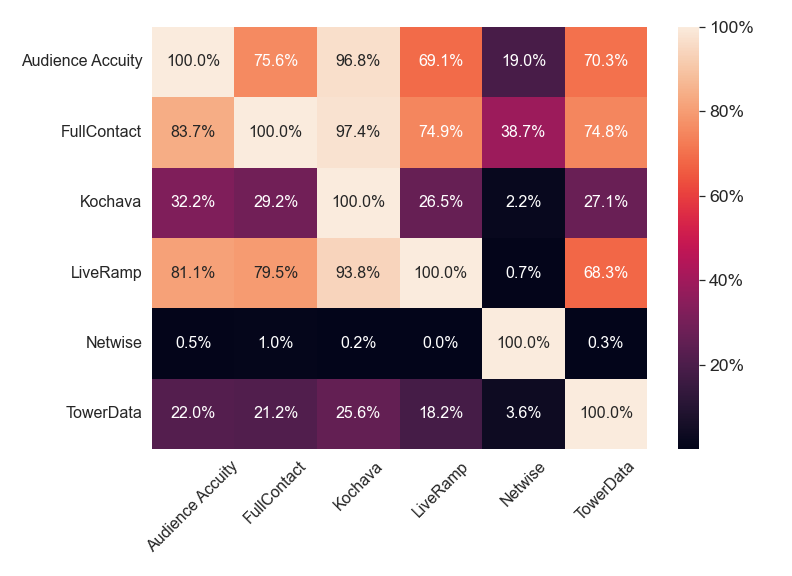
\includegraphics[width=0.8\linewidth]{../outputs/heatmap_percent_overlap.png}
  \caption{Overlapping percentage of the different identifiers covered by the licenses. The percentages relates to the volume of the license specified at the bottom of the column, i.e. the matrix should be read vertically.}
  \label{fig:heatmap_overlap}
\end{figure}

%section - Coverage of the licenses
\clearpage
\newpage
\section{Coverage of the licenses}
\begin{figure}[h!]
  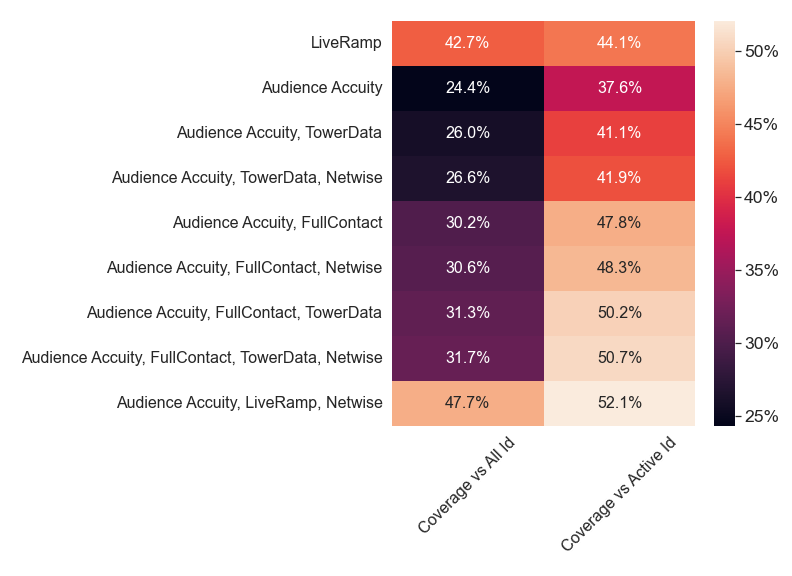
\includegraphics[width=0.7\linewidth]{../outputs/heatmap_percent_coverage.png}
  \caption{The percentage of coverage of the identifiers in the dataset considering all identifiers and only the ones that showed some activities for diverse combination of licenses sets.}
  \label{fig:heatmap_percent_coverage}
\end{figure}

\begin{figure}[h!]
  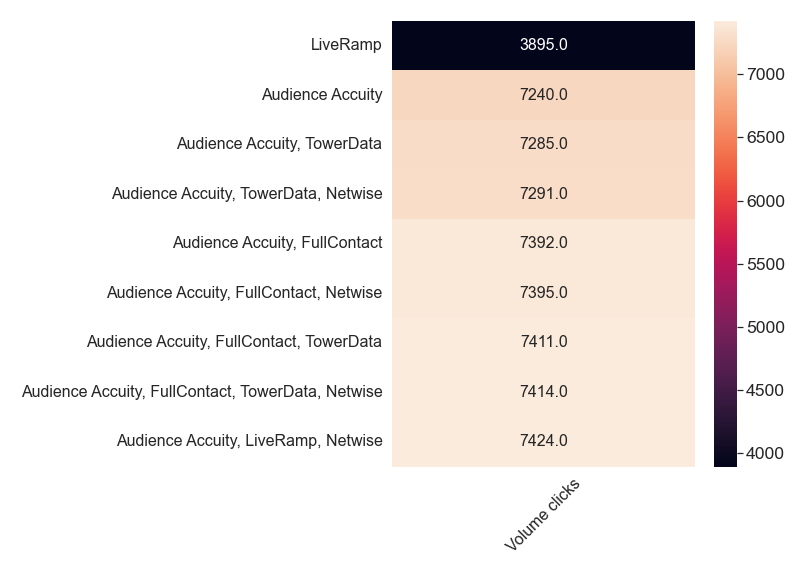
\includegraphics[width=0.7\linewidth]{../outputs/heatmap_volume_clicks.png}
  \caption{The number of clicks the set of license would be able to access}
  \label{fig:heatmap_vol_clicks}
\end{figure}

LiveRamp is covering 42.7\% of the identifiers of the dataset and 44.1\% of active identifiers (figure \ref{fig:heatmap_percent_coverage}). In comparison Audience Accuity is covering only 24.4\% of the dataset and 37.6\% of the active identifiers on its own.\\

\begin{minipage}[t]{0.45\linewidth}
  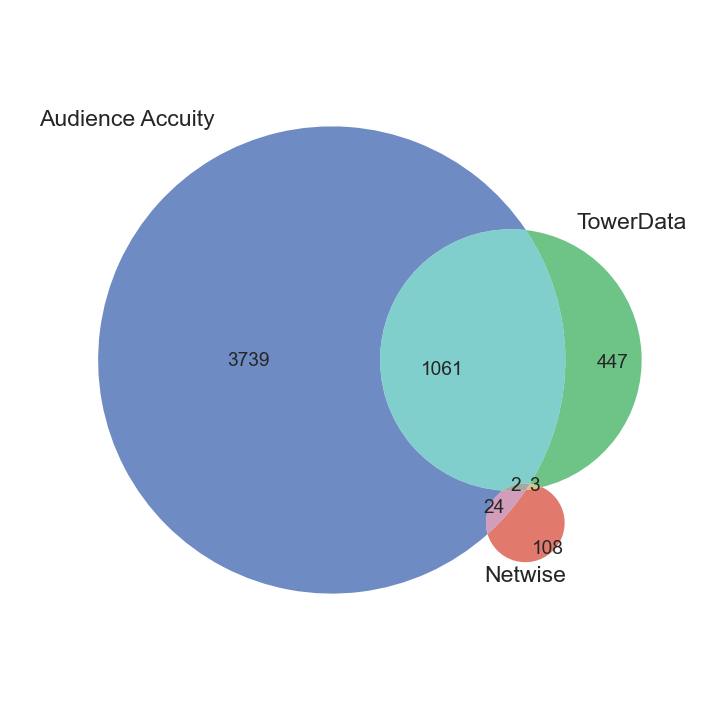
\includegraphics[width=1.1\linewidth]{../outputs/venn3_Audience Accuity_TowerData_Netwise.png}
  \captionof{figure}{The overlap between the Audience Accuity, TowerData and Netwise licenses}
  \label{fig:v3_AA_TD_N}
\end{minipage}\hfill
\begin{minipage}[t]{0.45\linewidth}
  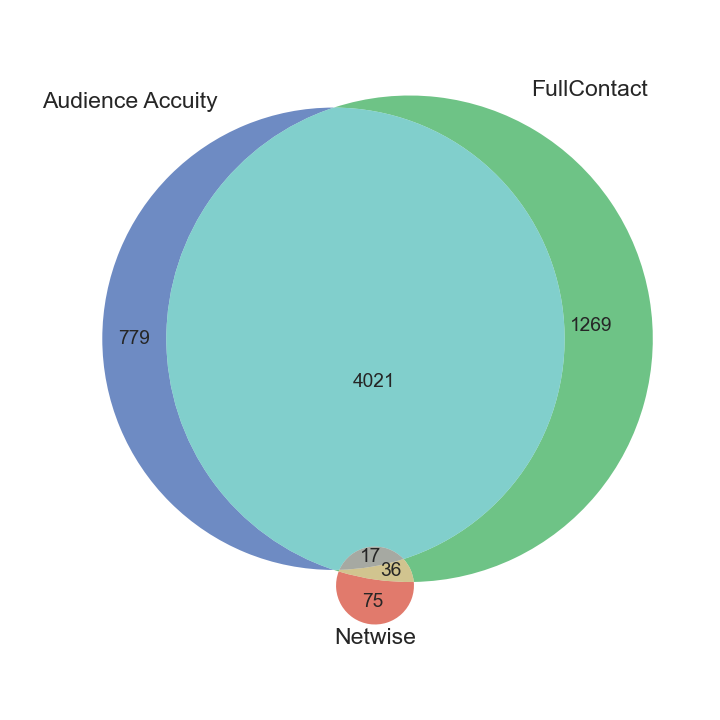
\includegraphics[width=1.1\linewidth]{../outputs/venn3_Audience Accuity_FullContact_Netwise.png}
  \captionof{figure}{The overlap between the Audience Accuity, FullContact and Netwise licenses}
  \label{fig:v3_AA_FC_N}
\end{minipage}

\begin{figure}[h!]
  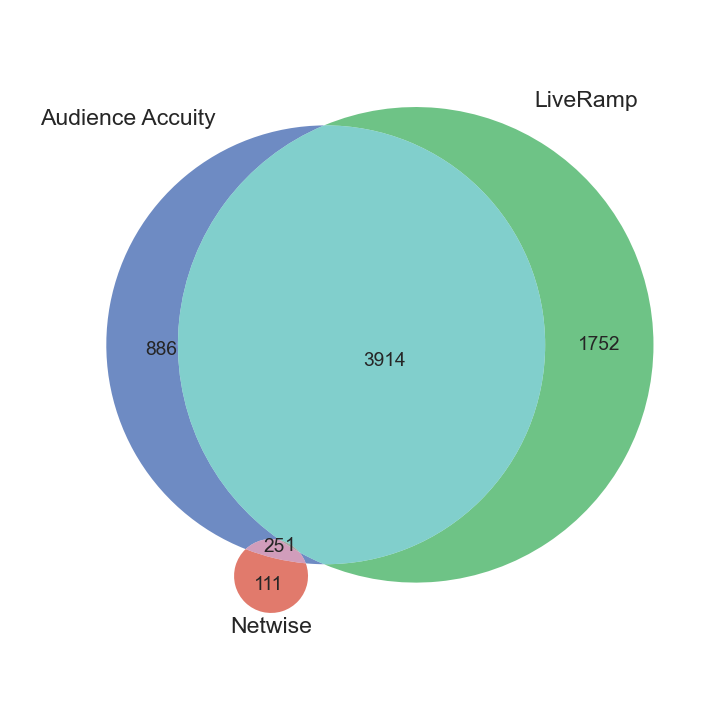
\includegraphics[width=0.48\linewidth]{../outputs/venn3_Audience Accuity_LiveRamp_Netwise.png}
  \caption{The overlap between the Audience Accuity, LiveRamp and Netwise licenses}
  \label{fig:v3_AA_LR_N}
\end{figure}

With the suggested set, Audience Accuity and TowerData, the licenses will cover 26.0\% of the identifiers, but 41.1\% of the active identifiers closing in on the LiveRamp's active coverage. Providing that the Netwise license is at a reasonable price, it could be added to the set to increase the coverage without maybe double coverage. The overlap between the three is fairly limited (figure \ref{fig:v3_AA_TD_N})\\

Another combination could be Audience Accuity, FullContact (with or without Netwise) which would bring more coverage, more clicks, however the overlap is fairly large (figure \ref{fig:heatmap_percent_coverage}, \ref{fig:heatmap_vol_clicks} and \ref{fig:v3_AA_FC_N}).\\

If the largest coverage is the most important, then a combination with Audience Accuity, LiveRamp and Netwise could bring a coverage over 50\% of the active identifiers but at the cost a very double coverage (figure \ref{fig:heatmap_percent_coverage}  and \ref{fig:v3_AA_LR_N}), and the increase number of clicks are marginal compared to other sets (figure \ref{fig:heatmap_vol_clicks}).
\end{document}
